% !TEX TS-program = LuaLaTeX

\documentclass[11pt,compress,xcolor=x11names,UTF8]{beamer}
\usetheme{Boadilla}
\usecolortheme{seahorse}
\useinnertheme[shadow]{rounded}
\useoutertheme[subsection=false]{smoothbars}
\usecolortheme{spruce}
\usecolortheme[named=SpringGreen4]{structure}
\usefonttheme{structurebold}
\useinnertheme{circles}
\usecolortheme{rose}
\usepackage{pifont}
\usepackage{academicons}
\usepackage{fontawesome}
\usepackage{iitem}
\usepackage{graphicx}
\usepackage{tabularx}
\setbeamertemplate{itemize item}{\ding{108}}
\setbeamertemplate{itemize subitem}{\ding{109}}
\setbeamertemplate{navigation symbols}{}
\setbeamercovered{transparent}
\renewcommand\appendixname{附录}
\renewcommand\abstractname{摘要}
\graphicspath{{figure/}} % 图片路径
\usepackage{calligra} % Thank you
\usepackage{ctex} % 加入中文
%\setCJKsansfont{Noto Sans CJK SC}
%\setsansfont{DejaVu} % Lato Roboto Fira Sans
\setsansfont{Lato} % Lato Roboto Fira Sans
\usepackage{makecell}
\newcommand{\tabincell}[2]{\begin{tabular}{@{}#1@{}}#2\end{tabular}}
\usepackage{url}
\usepackage{natbib} % 参考文献
%\title[Spatial Generalized Linear Mixed Models]{Spatial Generalized Linear Mixed Models with Application to Prevalence Mapping}
\title{Performance of CNN in PMT PDE Evaluation }
\subtitle{-- based on the onsite PMT testing data}
\author[Rong Zhao]{Email:zhaor25@mail2.sysu.edu.cn \and  } % \\ 专业:统计学 \\ 方向:数据分析与统计计算
\institute[SYSU]{School of Physics\and } % 理学院\\
\date[\today]{
\includegraphics[width=.5\textwidth]{logo}}
\begin{document}

\maketitle

\begin{frame}{Outline}
\tableofcontents
\end{frame}

\section{Brief Introduction}

%\subsection{研究意义}
%%%%%%%%%%%%%%%%%%%%%%%%%%%%%%%%%%%%%%%%%%%
% \begin{frame}{20 inch PMT}
% \begin{figure}
% \centering
% 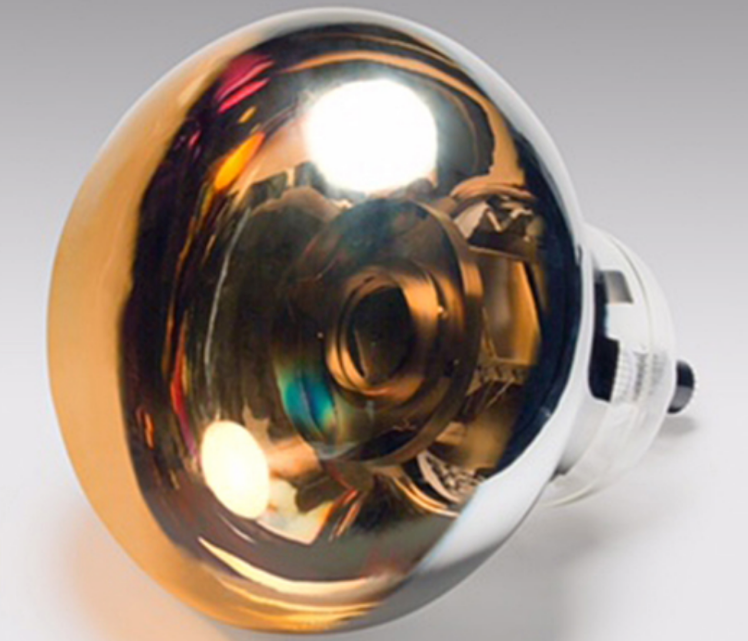
\includegraphics[width=0.60\textwidth]{figures/lpmt.png}
% \caption{20 inch PMT in JUNO CD}
% \end{figure}
% \end{frame}
%%%%%%%%%%%%%%%%%%%%%%%%%%%%%%%%%%%%%%%%%%%
\begin{frame}{traditional methods of PDE evaluation}
Calculate the expected p.e # by "cut" or "fiting" of chagre spectrum.
\begin{columns}
\begin{column}{.485\textwidth}
\begin{figure}
\centering
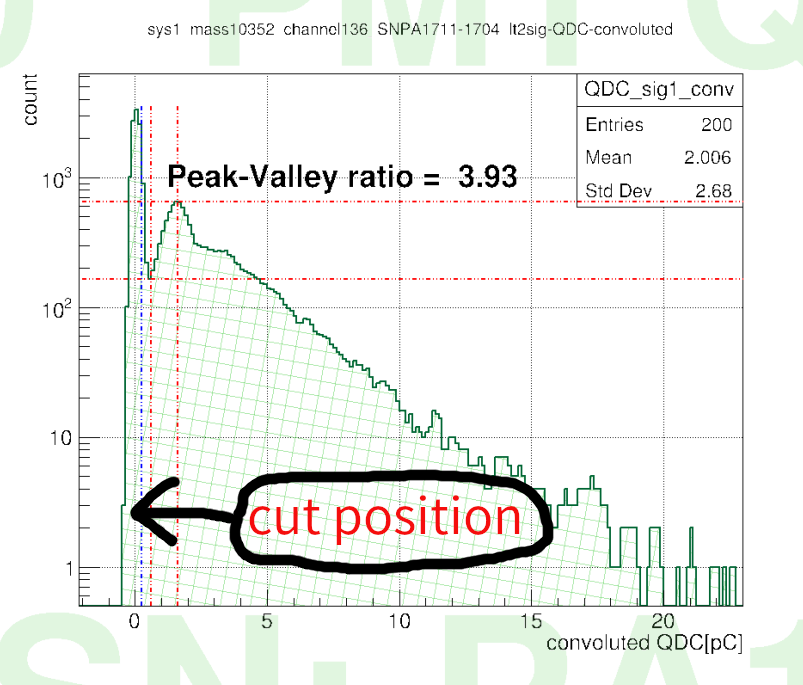
\includegraphics[width=\textwidth]{figure/specut.png} % 单图
%\label{fig:wave2d}
\caption{"cut" the charge spectrum to count pedestal events}
\end{figure}
\end{column}
\begin{column}{.5\textwidth}
\begin{figure}
\centering
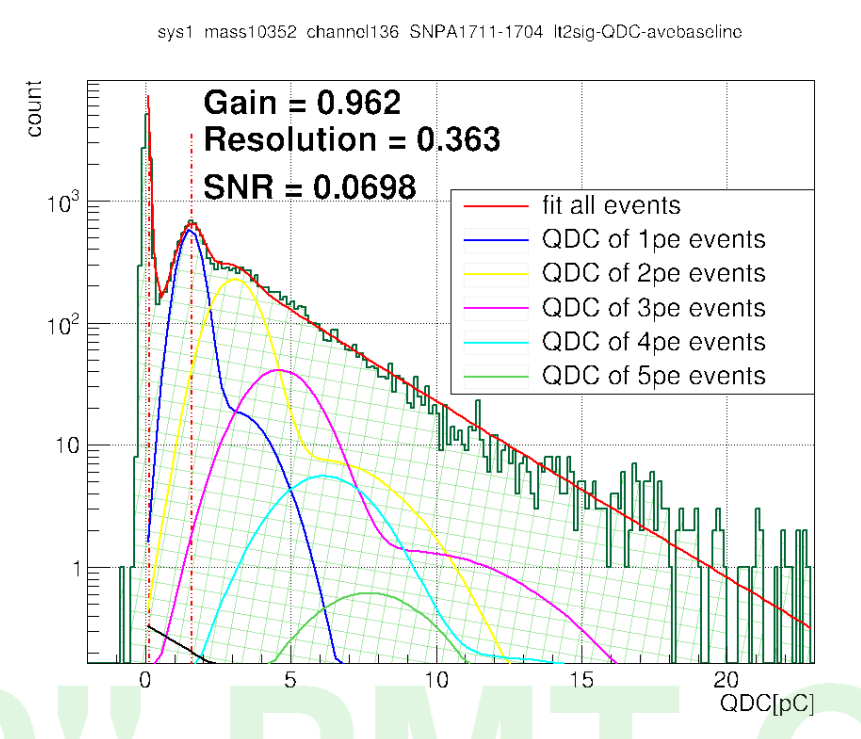
\includegraphics[width=\textwidth]{figure/spefit.png} % 单图
%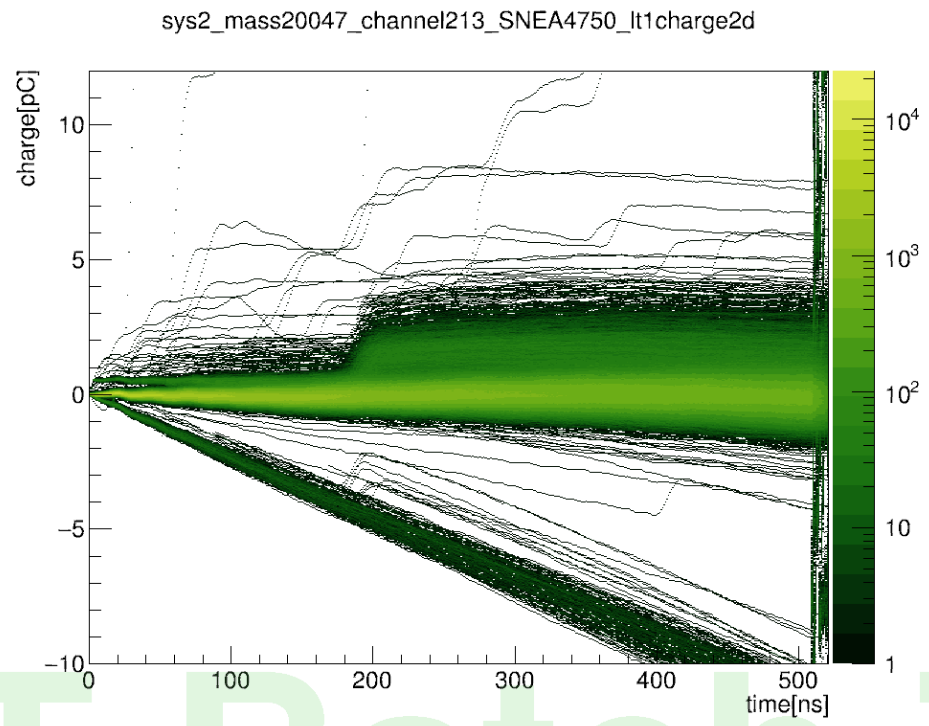
\includegraphics[width=\textwidth]{figures/baseline2d.png} % 单图
\caption{fit using a PMT photon response model}
\end{figure}
\end{column}
\end{columns}
\end{frame}
%\begin{frame}{waveform classification using CNN}
%We have tested \alert{5k HAMAMATSU PMTs} and about \alert{7k NNVT PMTs} in the container system. We can obtain the following  paramaters:
%\begin{table}[]
%\caption{PMT performance qualification standard}
%\resizebox{.8\textwidth}{!}{%
%\begin{tabular*}{.98\textwidth}{l|c|c}
%%\toprule
%\hline
%\hline
%parameter & HAMAMATSU PMT&NNVT PMT\\
%\hline
%HV@Gain=$10^7$ &  <2350 V&<2800V \\
% PDE & >24\%& >24\%\\
% DCR & <50kHz& <100kHz\\
% PV & >2.5& >2.5\\
% rise time & <8.5ns& --\\
% fall time & <12ns&-- \\
% FWHM & ----& --\\
% resolution & <0.4&<0.4 \\
%\hline
%\end{tabular*}
%}
%\end{table}
%\alert{The Main aim of testing data analysis is to evaluate theses parameters and check wave quality of one PMT.}
%%\begin{figure}
%%\centering
%%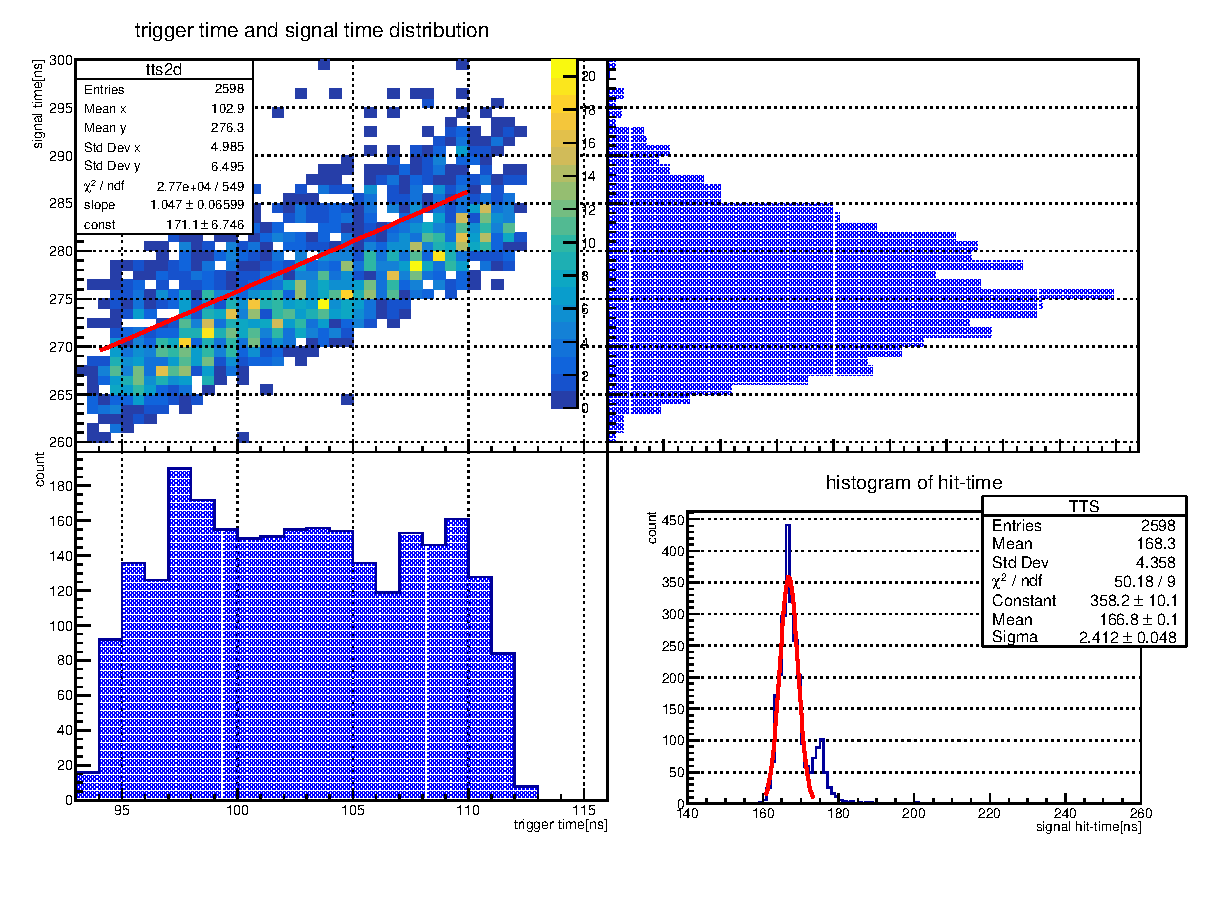
\includegraphics[width=0.78\textwidth]{typical_hittime} % 单图
%%\end{figure}
%\end{frame}
%%%%%%%%%%%%%%%%%%%%%%%%%%%%%%%%%%%%%%%%%%%%
%\begin{frame}{Flowchart of analysis procedure}
\begin{frame}{waveform classification using CNN}
CNN can perform a powerful PSD and classify the waveforms, then we could get explicit p.e# during one test.   
\begin{columns}
\begin{column}{.485\textwidth}
\begin{figure}
\centering
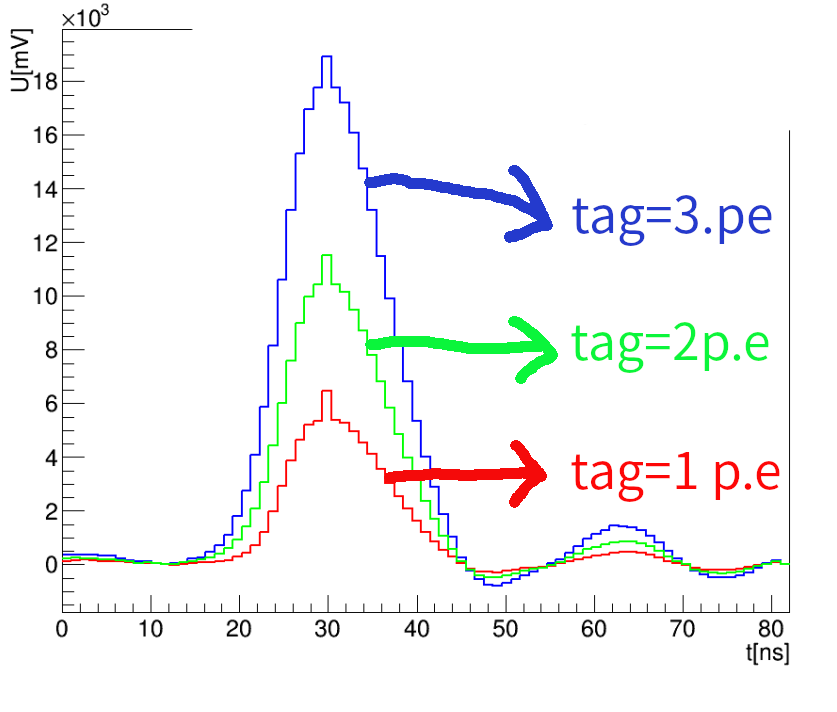
\includegraphics[width=0.94\textwidth]{figure/cnntags.png} % 单图
\caption{tags of typical waveform from CNN}
\end{figure}
\end{column}
\begin{column}{.485\textwidth}
\begin{figure}
\centering
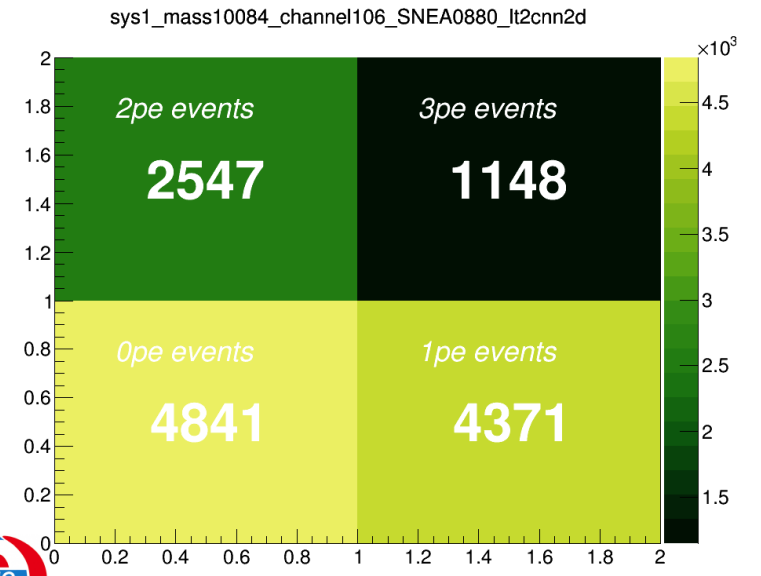
\includegraphics[width=0.94\textwidth]{figure/cnnres.png} % 单图
\caption{classification of events in one test}
\end{figure}
\end{column}
\end{columns}

\end{frame}
%%%%%%%%%%%%%%%%%%%%%%%%%%%%%%%%%%%%%%%%%%%
\begin{frame}{ the expected photon number}
	If we do a "cut" is the charge spectrum@0.25 spe, the averager photon number $\mu$ can be acquired by\footnote{E. H. Bellamy et al /Nucl. Instr. and Meth. m Phys . Res. A 339 (1994) 468-476}
\begin{equation}
	\mu=-ln(\frac{N_{0}}{N})
\end{equation}
	where $N_{0}$ is the number of pedestal(0 p.e) events, N is the total event number.
\vspace{.3cm}
\hrule{\textwidth}
\vspace{.3cm}
However, if we know explicitly the photon number of specific event, the $\mu$ value is :
\begin{equation}
	\mu=1\times n_{1}+2\times n_{2}+\cdot\cdot\cdot+N\times n_{N}
\end{equation}
	where $n_{N}$ is the number of N p.e events.
\end{frame}
%%%%%%%%%%%%%%%%%%%%%%%%%%%%%%%%%%%%%%%%%%%
%\begin{frame}{PMT testing report-pass}
%We have generated testing report for each qualified PMT.
%\vspace{-.2cm}
%\begin{figure}
%\centering
%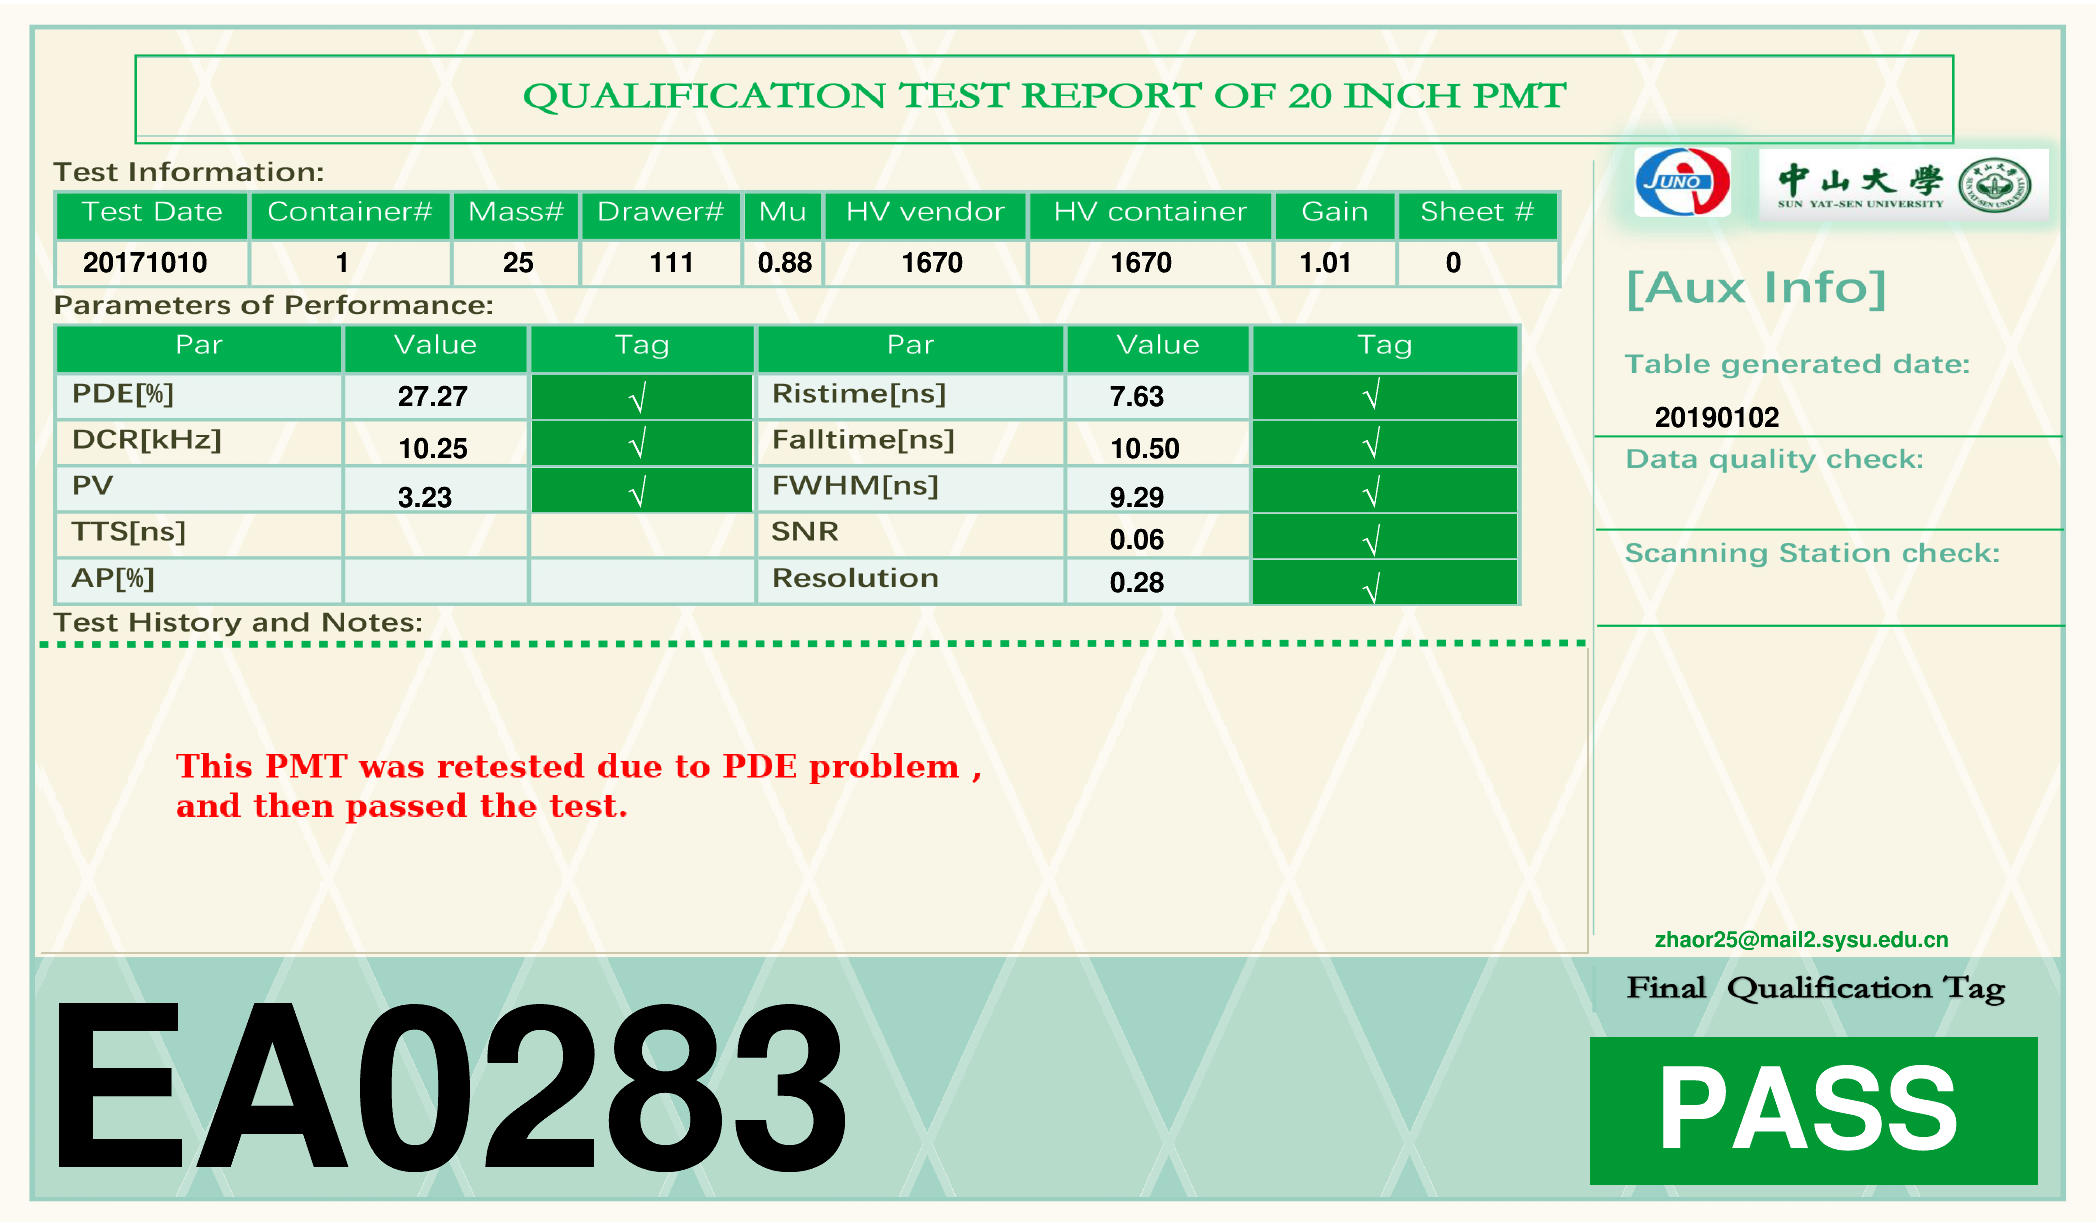
\includegraphics[width=1.0\textwidth]{figures/SN_EA0283_pde1_dcr1_HV1_pv1_rt1_tag1.png}
%\end{figure}
%\end{frame}
%%%%%%%%%%%%%%%%%%%%%%%%%%%%%%%%%%%%%%%%%%%
%\begin{frame}{calibration of each drawer}
%Generally, we put several PMTs with known PDE value\footnote{or QE value}  into one drawer and linearly fit the PDE-$\mu_{test}$ data to get \alert{drawer$_{factor}$}.
%\vspace{.5cm}
%\hrule{\textwidth}
%\vspace{.5cm}
%
%While an alternative way to access the drawer$_{factor}$ is fitting PDE-$\mu_{test}$ data {\color{red}from all the PMTs tested in one drawer rather than the mannual selected ones.} Then once we finish one PMT test in a drawer we will get one more statistical sample in the PDE-$\mu_{test}$ fitting, and we could expect that the fitted drawer$_{factor}$ will get more stable as we testing more PMTs.
%
%\vspace{.5cm}
%The advantage of this "self-calibration" method is that we could {\color{red}decrease the statistical error as much as possible}; and the remained fluctuation of drawer$_{factor}$ can be the system error.
%\end{frame}
\section{traing and test of CNN}
%%%%%%%%%%%%%%%%%%%%%%%%%%%%%%%%%%%%%%%%%%%
\begin{frame}{input of CNN}
slecet  
\end{frame}
%%%%%%%%%%%%%%%%%%%%%%%%%%%%%%%%%%%%%%%%%%%
%\begin{frame}{一个抽屉的刻度结果}
%随着测试PMT数量的增加,拟合统计误差逐渐减小,$drawer_{factor}$的拟合结果趋于稳定(更多抽屉拟合结果见back-up部分)。
%\begin{figure}
%\centering
%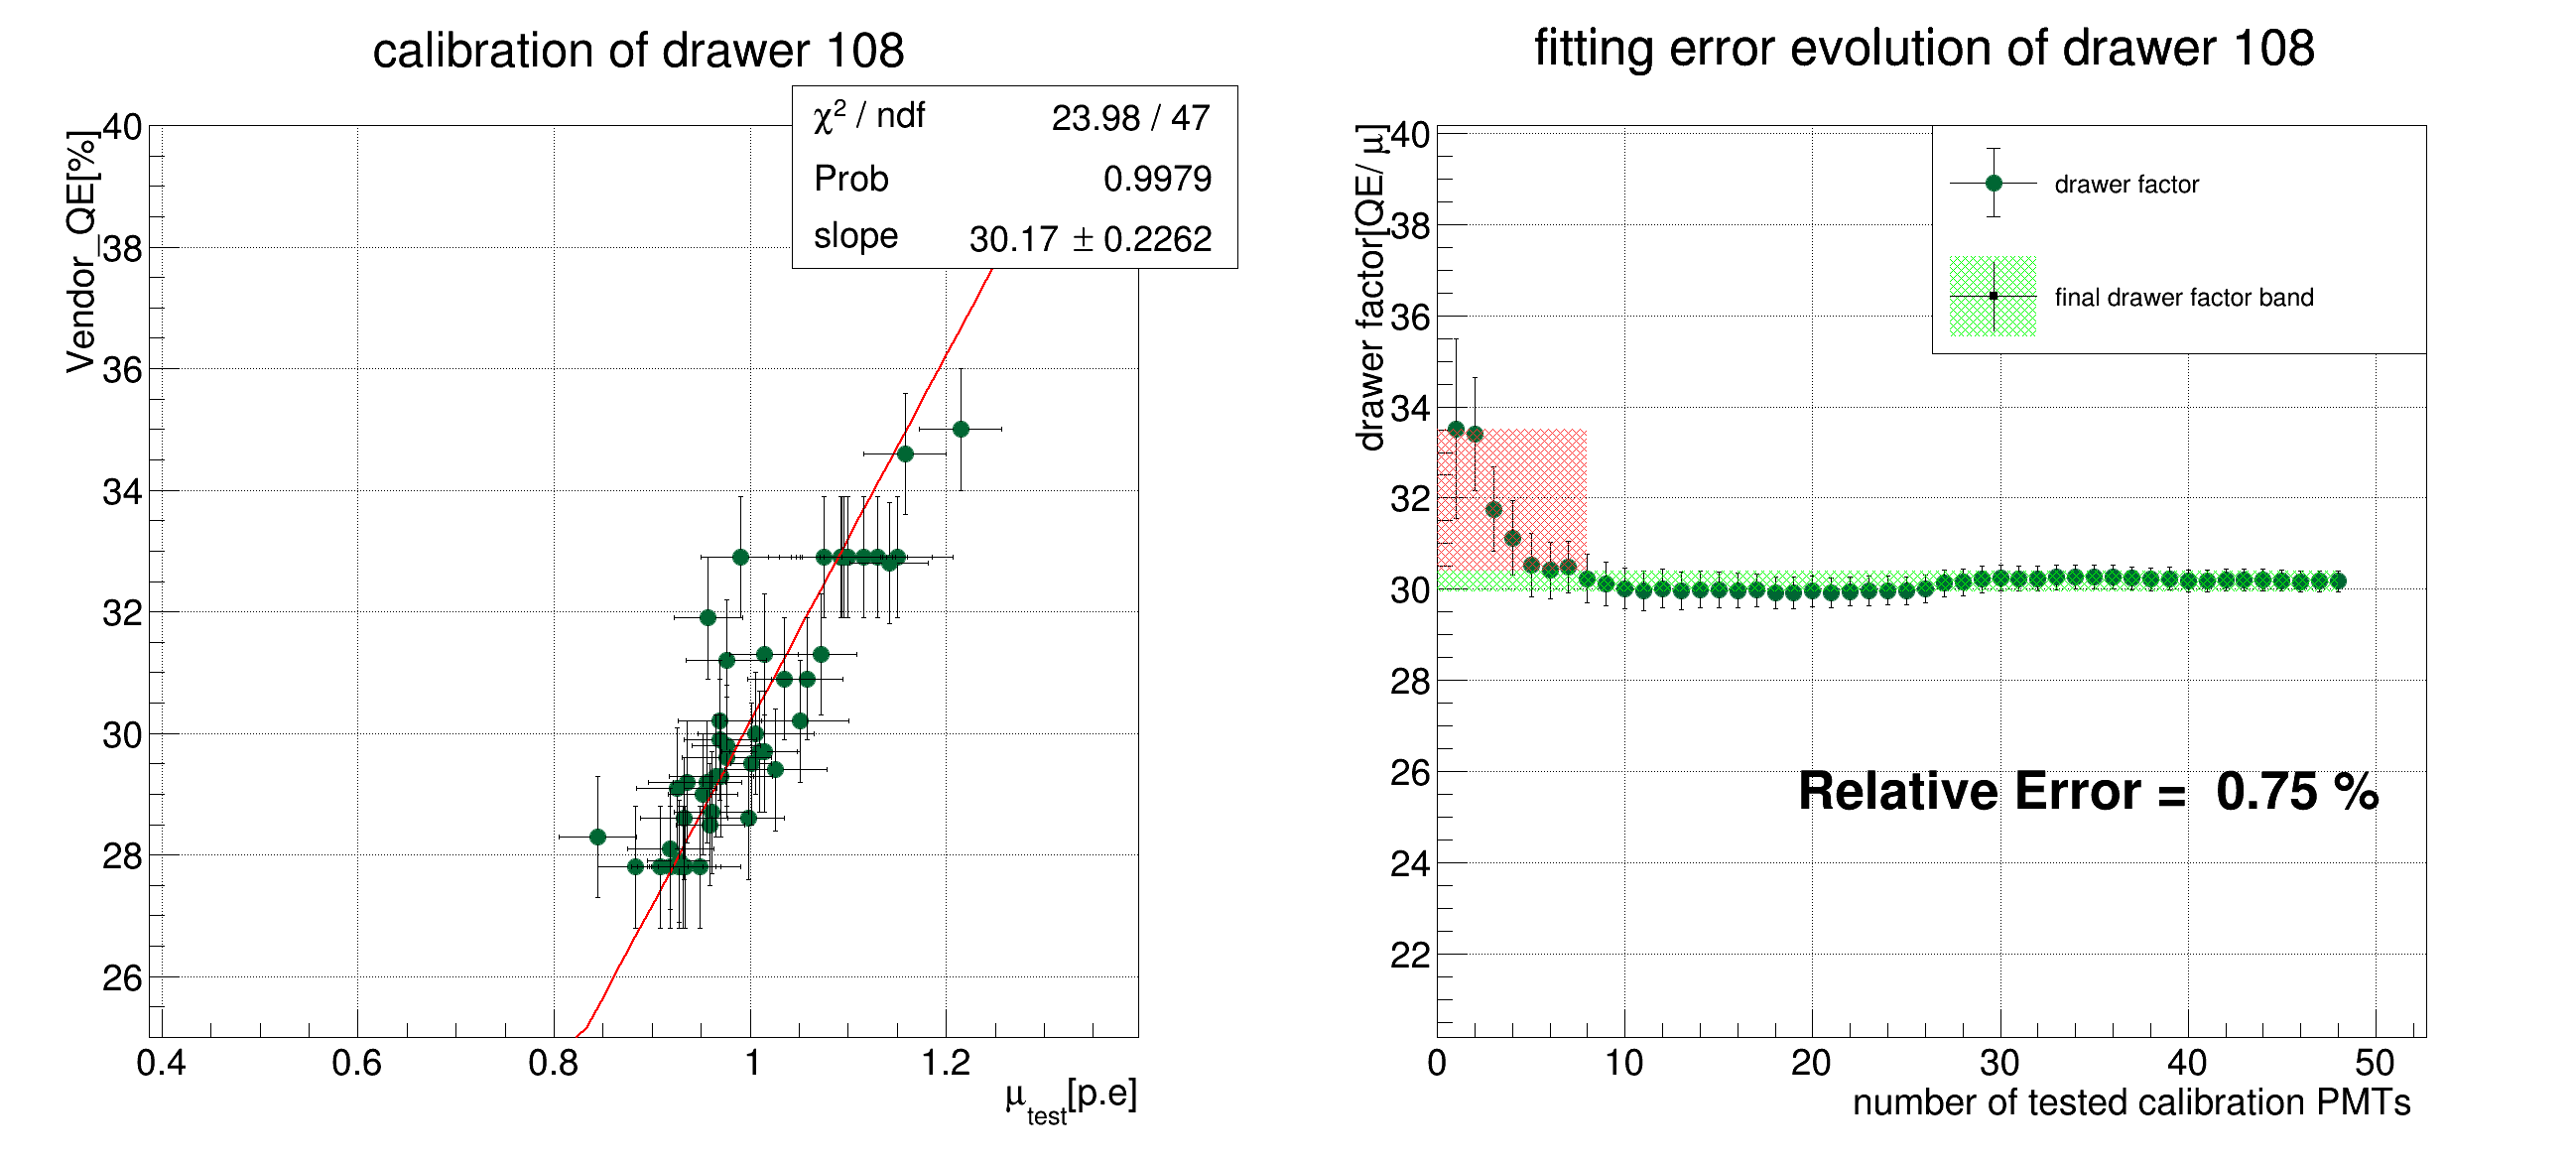
\includegraphics[width=0.98\textwidth]{sta101-7} % 单图
%\caption{108抽屉的$drawer_{factor}$拟合结果}
%\end{figure}
%\end{frame}
%%%%%%%%%%%%%%%%%%%%%%%%%%%%%%%%%%%%%%%%%%%
%~~!!!!!!!!!!!!!!!!!!put two figures to illustrate!!!!!
\begin{frame}{Output waveforms of PMT @$Gain=10^7$}
The 2-D waveform histogram contains all the recorded waveforms, we can clearly see the "delayed signals" of HAMMATSU PMT and "big signals" of NNVT PMTs.
\begin{columns}
\begin{column}{.47\textwidth}
\begin{figure}
\centering
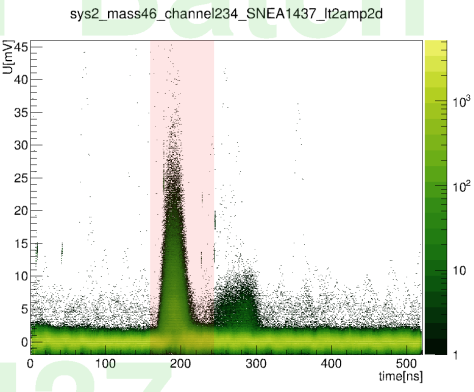
\includegraphics[width=\textwidth]{figures/wave2d.png} % 单图
%\label{fig:wave2d}
\caption{all frames of HAMAMATSU PMT}
\end{figure}
\end{column}
\begin{column}{.5\textwidth}
\begin{figure}
\centering
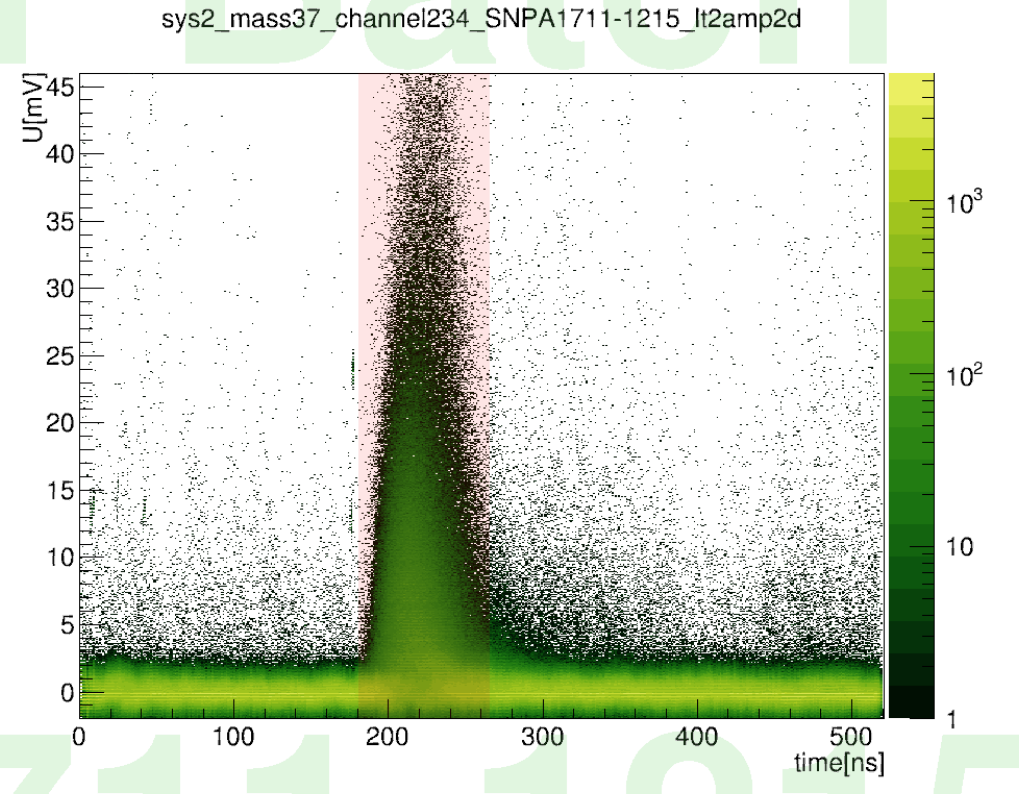
\includegraphics[width=\textwidth]{figures/mcpwave2d.png} % 单图
%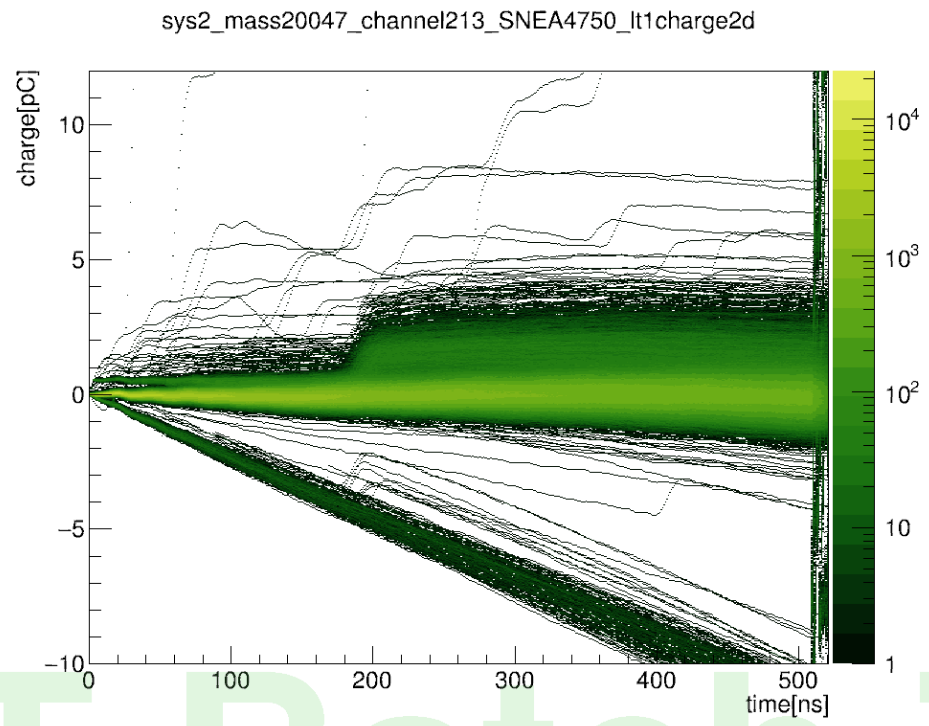
\includegraphics[width=\textwidth]{figures/baseline2d.png} % 单图
\caption{all frames of NNVT PMT}
\end{figure}
\end{column}
\end{columns}
\end{frame}
%%%%%%%%%%%%%%%%%%%%%%%%%%%%%%%%%%%%%%%%%%%
%%%%%%%%%%%%%%%%%%%%%%%%%%%%%%%%%%%%%%%%%%%
%%%%%%%%%%%%%%%%%%%%%%%%%%%%%%%%%%%%%%%%%%%
%\section{参数计算和结果分析}
%%%%%%%%%%%%%%%%%%%%%%%%%%%%%%%%%%%%%%%%%%%%%%%%%%%%%%
%%%%%%%%%%%%%%%%%%%%%%%%%%%%%%%%%%%%%%%%%%%%%%%%%%%%%%
%~~!!!!!!!!!!!!!!!!!!put two figures to illustrate!!!!!
%\begin{frame}{抽屉刻度结果分析\footnote{拟合出的抽屉因子与现场所使用的抽屉因子的关联见back-up部分}}
%\begin{columns}
%\begin{column}{.5\textwidth}
%\begin{figure}
%\centering
%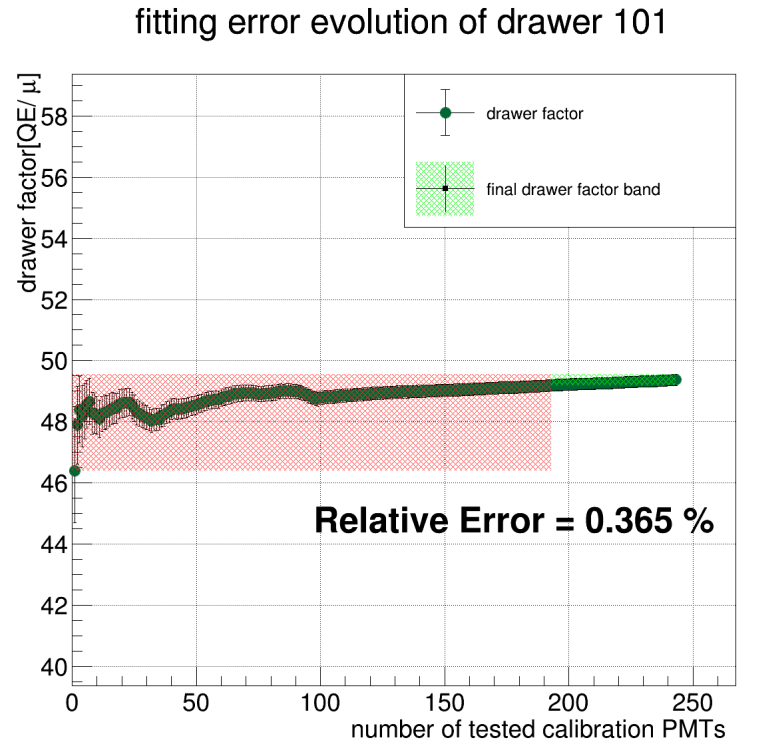
\includegraphics[width=\textwidth]{lt101} % 单图
%\end{figure}
%\end{column}
%\begin{column}{.45\textwidth}
%101抽屉一直放置参考PMT EA0419,抽屉因子$drawer_{factor}$拟合的结果随着时间漂移,这存在两种可能:
%\vspace{.5cm}
%
%\hrule{\textwidth}
%\vspace{.5cm}
%
%另一方面,这样的刻度方法可以用来监控系统的稳定性。因为如果系统稳定工作,拟合系数应该随机涨落。
%
%\end{column}
%\end{columns}
%\end{frame}
%%%%%%%%%%%%%%%%%%%%%%%%%%%%%%%%%%%%%%%%%%%
%%%%%%%%%%%%%%%%%%%%%%%%%%%%%%%%%%%%%%%%%%%%%%%%%%%%%%
%%%%%%%%%%%%%%%%%%%%%%%%%%%%%%%%%%%%%%%%%%%
\begin{frame}{calculation of $PDE$}
we can obtain the average photon number $\mu_{test}$ from charge spectrum, along with the $drawer_{factor}$\footnote{Calibrate the drawer factor using PMT tested in the drawer which has vendor QE value.}, the PDE result from container system is:
\begin{equation}
PDE_{c}=\mu_{test}\times drawer_{factor}
\end{equation}
Then we map the PDE from container to the final PDE value with the help of container $f_{cs}$\footnote{linear correlation factor}:
\begin{equation}
PDE=PDE_{c}.f_{cs}+constant
\label{pde_formula}
\end{equation}
%根据公式\ref{pde_formula},通过$\mu_{test}$以及抽屉因子即可算出集装箱自己的PDE结果$PDE_c$。假设集装箱系统和扫描站对同一只PMT的测量结果是正比关系\footnote{参考王俊和王耀光的模拟结果},通过拟合线性参数$f_{cs}$可以算出最终的PDE。
\vspace{.5cm}
\hrule{\textwidth}
\vspace{.5cm}

\end{frame}
%%%%%%%%%%%%%%%%%%%%%%%%%%%%%%%%%%%%%%%%%%%
\begin{frame}{statistical results}
Mean value of parameters for HAMAMATSU-PMT and NNVT-PMT\footnote{For the parameter TTS, we need to test the internal time resolution firstly, since we found the TTS results is highly drawer related.}:

\vspace{.5cm}

\centering
\begin{tabular}{l|c|c}
\hline
\hline
parameters(mean)&  {\color{Blue} HAMAMATSU} & {\color{Blue}NNVT} \\\hline
DCR(kHz)&15.38&41.24\\
rise time(ns)&7.4& 3.2\\
fall time(ns)&10.36& 15.9\\
PV&3.39& 3.19\\
resolution&0.28& 0.35\\
HV@1E7(V)&1861& 1783\\
FWHM(ns)&9.08& 5.8\\
\hline
\end{tabular}
\end{frame}
%%%%%%%%%%%%%%%%%%%%%%%%%%%%%%%%%%%%%%%%%%%%%%%%%%%%%%
\section{Summary}
\begin{frame}{summary}
\begin{itemize}
\item  the charge and amplitude stability of HAMAMATSU PMT is better.
\item  $\sim$6k NNVT PMTs and 5k HAMAMATSU PMTs has been tested in container system, test results and test reports are avaliable from PMTDataBase\footnote{pmtdb.juno.ihep.ac.cn}.
\item we reject or accept one PMT according to its perfomance test results from container and scanning station.
\item  {\color{red}we need to study the "delay signal" of HAMAMATSU PMT and "big signal" of NNVT PMT\footnote{especially when PMT working in the multi-photon case}} in detail\footnote{one option is to transport several PMTs to SYSU for detailed study}.
\item the expected mean PDE value is 30.4\% and mean DCR value is $\sim$34kHz\footnote{will decrease after installation} in CD.
%\item 保存重要的测试信息和输出结果到PMT数据库,所有测试结果\footnote{包含集装测试历史数据}可以直接通过http://pmtdb.juno.ihep.ac.cn/\footnote{Query::LPMT Tested Reports} 查询得到
%\item 初步结论:目前现场5002支滨松PMT,382支外观检测不合格,5支HV不合格,2支波形较差,24支DCR不合格,9支PDE不合格。
\end{itemize}
\end{frame}

\begin{frame}
\centering {\zihao{0} \color{red} {THANKS}}
\end{frame}

\begin{frame}
\centering {\zihao{0} \color{red} {BACK-UP}}
\end{frame}

%\begin{table}[htbp]
%\caption{PMT typical performance}
%\resizebox{.8\textwidth}{!}{%
%\begin{tabular*}{.98\textwidth}{l|cccc}
%%\toprule
%\hline
%\hline
%Performance & PDE &DCR & TTS& uniformity \\
%\hline
%HAMAMATSU &  lower\% & 20 kHz& 3ns& worse \\
%NNVT  & higher\% & 40kHz & 7ns& better \\
%\hline
%\end{tabular*}
%%}
%\end{table}

%\end{frame}
%%%%%%%%%%%%%%%%%%%%%%%%%%%%%%%%%%%%%%%%%%%%%%%%%%%%%%
\begin{frame}{TTS of HAMAMATSU PMT}
\begin{figure}
\centering
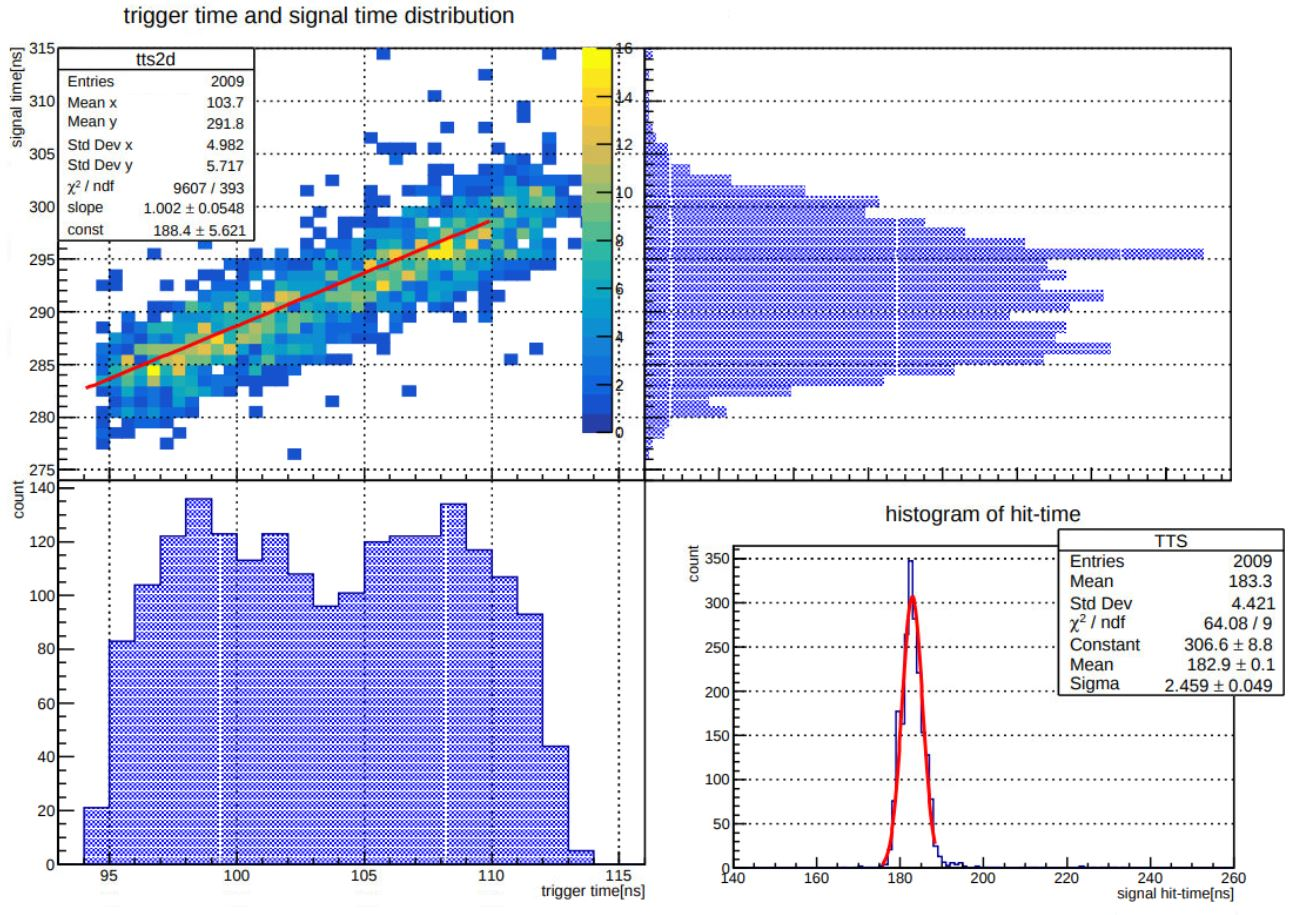
\includegraphics[width=.8\textwidth]{figures/hamtts.JPG} % 单图
%\label{fig:wave2d}
\caption{hittime and trigger time}
\end{figure}
\end{frame}
%%%%%%%%%%%%%%%%%%%%%%%%%%%%%%%%%%%%%%%%%%%%%%%%%%%%%%
\begin{frame}{TTS calculation of NNVT PMT}
\begin{figure}
\centering
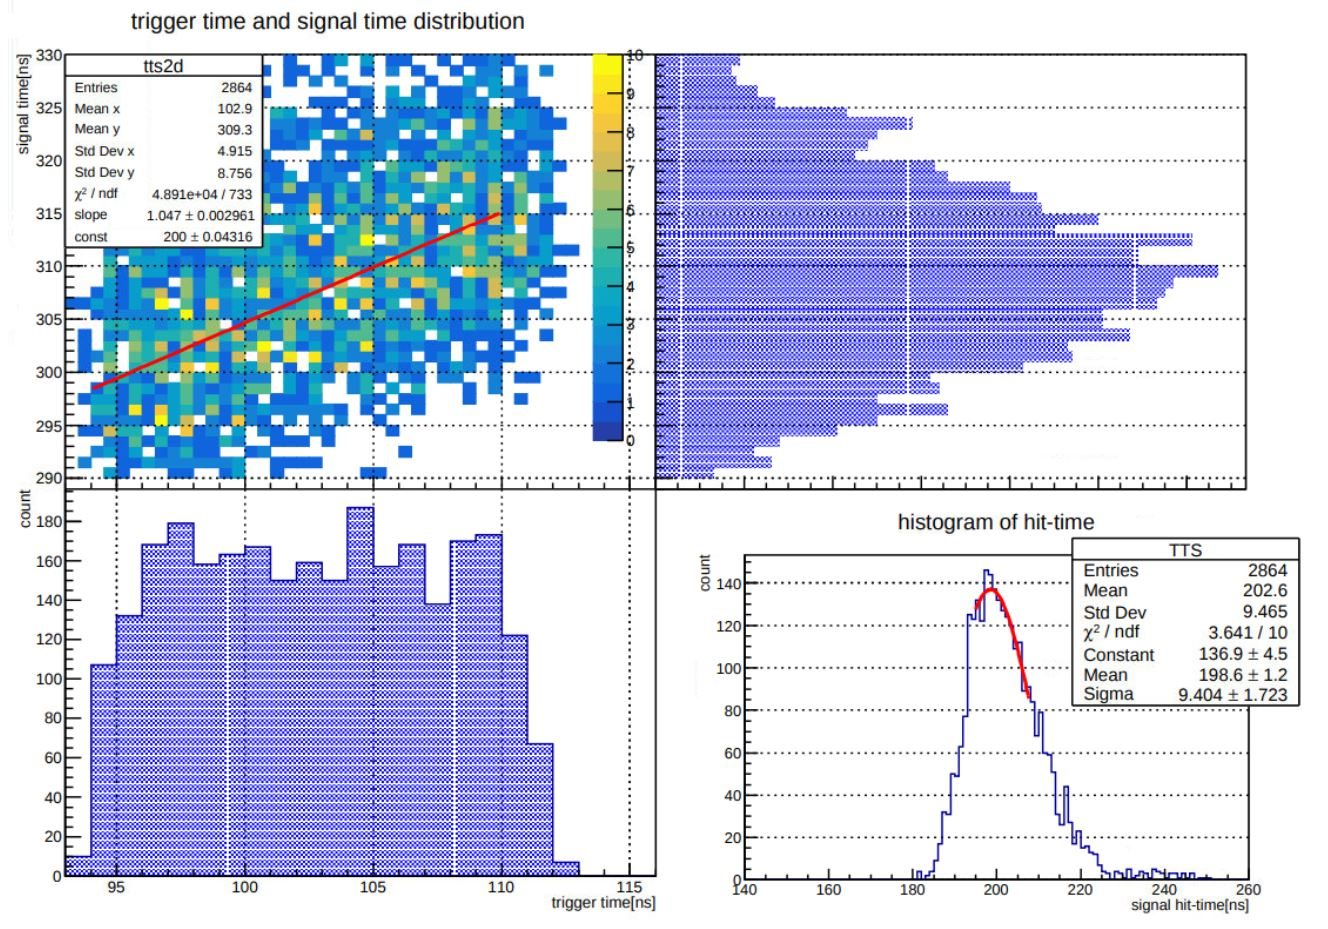
\includegraphics[width=.8\textwidth]{figures/mcptts.JPG} % 单图
%\label{fig:wave2d}
\caption{hittime and trigger time}
\end{figure}
\end{frame}
%%%%%%%%%%%%%%%%%%%%%%%%%%%%%%%%%%%%%%%%%%%
\end{document}
